\documentclass[%handout,
11pt,a4paper,xcolor={usenames,dvipsnames}]{beamer}
\setbeamertemplate{navigation symbols}{}
\usepackage{lgdv/beamerthemetest}
\usepackage[utf8]{inputenc}
\usepackage{amsmath}
\usepackage{amsfonts}
\usepackage{amssymb}
\usepackage{graphicx}
\usepackage{caption}
\usepackage{subfig}
\usepackage{array}
\usepackage{tabularx}
\usepackage{listings}
\usepackage{multicol}
\usepackage{changepage}

\definecolor{mygreen}{rgb}{0,0.6,0}
\definecolor{mygray}{rgb}{0.5,0.5,0.5}
\definecolor{mymauve}{rgb}{0.58,0,0.82}

\lstset{
	basicstyle=\ttfamily\normalsize,
	language=Python,
	keywordstyle=\color{mygreen},
	showspaces=false,
	showstringspaces=false,
	stringstyle=\color{mymauve},
	commentstyle=\normalfont\color{mygray},
	keepspaces=true,
	columns=fullflexible,
}
\captionsetup[subfloat]{labelformat=empty}
\captionsetup[figure]{labelformat=empty}
\captionsetup[table]{labelformat=empty}


\setlength{\columnsep}{0.1cm}
\setcounter{tocdepth}{2}

%% Hier ändern
\author{Jennifer Kane, Jonas Gröger}
\date{\today}

\begin{document}
    \begin{frame}[plain]
    \title{Informationsvisualisierung}
	\subtitle{Übungspräsentation}
	\titlepage
    \end{frame}

    % 3.1 Visuelle Eigenschaften...
    \begin{frame}{3.1 Visuelle Eigenschaften von Graphen}{Layout}
        \begin{itemize}
            \item \textbf{Arten:} hierarchische, kreisförmige, kraftbasiert
            \item \textbf{Beispiel:} GPS-Rohdaten $\rightarrow$ POIs $\rightarrow$ Werbung
            \item \textbf{Begründung:} Isomorphie von kraftbasierten Graphen wird ausgenutzt: Orte nicht Laufwege für Werbung interessant
        \end{itemize}
    \end{frame}

    \begin{frame}{3.1 Visuelle Eigenschaften von Graphen}{Visuelle Codierung}
        \begin{itemize}
            \item \textbf{Arten:} Form, Größe und Farbe eines Knoten / einer Kante
            \item \textbf{Beispiel:} Viele Freunde $\rightarrow$ großer Knoten
            \item \textbf{Begründung:} Visuell schnell aufzufassen
        \end{itemize}
    \end{frame}

    \begin{frame}{3.1 Visuelle Eigenschaften von Graphen}{Rendering}
        \begin{itemize}
            \item \textbf{Arten:} Interaktion im Allgemeinen
            \item \textbf{Beispiel:} Warmwasserleitungen zwischen Städten (Übersicht) und innerhalb einzelner Städte (Detailansicht) durch zoomen erfahrbar
            \item \textbf{Begründung:} Ansicht auf geeignetem Abstraktionsniveau
        \end{itemize}
    \end{frame}

    \begin{frame}{3.1 Visuelle Eigenschaften von Graphen}{Vereinfachung}
        \begin{itemize}
            \item \textbf{Arten:} Cluster, collapsing, Hierarchien
            \item \textbf{Beispiel:} Dateisysteme, z.B. Finder, Nautilus, Explorer
            \item \textbf{Begründung:} Ansicht auf geeignetem Abstraktionsniveau
        \end{itemize}
    \end{frame}

    % Visualisierungen benutzen immer mehrere dieser Elemente.

    \begin{frame}{3.2 Visual Clutter}{Kamada-Kawai - Rahmenbedingungen}
        \begin{itemize}
        	\item ungerichtete, gewichtete Graphen
        	\item gerade Kanten, keine Beschränkung bei Positionierung der Knoten
        	\item zusammenhängender Graph (sonst: Zusammenhangskomponenten einzeln zeichnen)
    	\end{itemize}
    \end{frame}

    \begin{frame}{3.2 Visual Clutter}{Kamada-Kawai - Kriterien}
        \begin{itemize}
        	\item Anzahl Kantenkreuzungen reduzieren
        	\item gleichmäßige Verteilung von Knoten und Kanten (wichtiger für menschliches Verständnis)
    	\end{itemize}
    \end{frame}

    \begin{frame}{3.2 Visual Clutter}{Kamada-Kawai - Idee}
        \begin{itemize}
        	\item Stahlringe werden durch Federn zusammengehalten
        	\item Ziel: Minimierung der Energie dieses Systems
        	\item ideale Distanz zwischen zwei Knoten proportional zur Länge eines kürzesten Pfades zwischen ihnen
    	\end{itemize}
    \end{frame}

    \begin{frame}{3.2 Visual Clutter}{Kamada-Kawai - Algorithmus}
        \begin{itemize}
        	\item Berechnung der Distanz $d_{i,j}$  (Shortest Path Algorithm - Floyd), in gewichteten Graphen: Distanz = Summe der Gewichte
        	\item Berechnung der Länge $l_{i,j}$ (aus Distanz und optimaler Länge)
        	\item Berechnung der Federstärke $k_{i,j}$ (aus Distanz)
        	\item Bestimmung der initialen Knotenpositionen
        	\item Schrittweise Minimierung der Energie: Verschieben eines Knotens in stabile Position
    	\end{itemize}

    	Laufzeit: O($|V|^3 + T * |V|$), $T =$ Anzahl der Iterationen
    \end{frame}

    \begin{frame}{3.2 Visual Clutter}{Kamada-Kawai - Ergebnisse}
        \begin{itemize}
        	\item symmetrische Graphen werden auch symmetrisch angeordnet
        	\item isomorphe Graphen werden auf dieselbe Art und Weise dargestellt (evtl. verschoben, gedreht oder gespiegelt)
    	\end{itemize}
    \end{frame}

    % Rheingold

    \begin{frame}{3.2 Visual Clutter}{Fruchtermann-Reingold - Rahmenbedingungen}
        \begin{itemize}
        	\item ungerichtete Graphen
        	\item gerade Kanten, Graph begrenzt durch festen Rahmen
    	\end{itemize}
    \end{frame}

    \begin{frame}{3.2 Visual Clutter}{Fruchtermann-Reingold - Kriterien}
        \begin{itemize}
        	\item gleichmäßige Verteilung von Knoten und Kanten innerhalb des Rahmens
        	\item Anzahl Kantenkreuzungen reduzieren
        	\item Streben nach symmetrischer Darstellung
        	\item Nachbarknoten sollen nah beieinander liegen, Knoten sollen aber nicht zu eng zusammen gezeichnet werden
    	\end{itemize}
    \end{frame}

    \begin{frame}{3.2 Visual Clutter}{Fruchtermann-Reingold - Idee}
        \begin{itemize}
        	\item Knoten verhalten sich wie Atomteilchen und üben anziehende und abstoßende Kräfte aufeinander aus
        	\item zur Vereinfachung: anziehende Kräfte nur zwischen Nachbarknoten, abstoßende Kräfte zwischen allen Knoten
        	\item Geschwindigkeit statt Beschleunigung, statisches Gleichgewicht statt dynamischem Gleichgewicht
    	\end{itemize}
    \end{frame}

    \begin{frame}{3.2 Visual Clutter}{Fruchtermann-Reingold - Algorithmus}
        \begin{itemize}
        	\item Berechnung der abstoßenden Kräfte
	        \item Berechnung der anziehenden Kräfte
	        \item Verschiebung begrenzen durch Temperatur
	        \item Teilchen am Rahmen stoppen
	        \item Sonderfall: zwei Knoten mit derselben Position $\rightarrow$ behandeln als wären sie dicht beieinander, dann wirken große abstoßende Kräfte
    	\end{itemize}

    	Laufzeit: O(T * ($|V|^2 + |E| + |V||E|$)),
    	
    	 $T =$ Anzahl der Iterationen $=$ O($|V|$) oder O($|E|$)
    \end{frame}

    \begin{frame}{3.2 Visual Clutter}{Fruchtermann-Reingold - Algorithmus (Variante)}
        \begin{itemize}
        	\item Einteilung in Gitter
        	\item abstoßende Kräfte nur zwischen Knoten benachbarter Quadrate
        	\item besser: abstoßende Kräfte zwischen Knoten innerhalb eines Kreises um Ausgangsknoten
    	\end{itemize}

    	Laufzeit: O(T * ($|V| + |E| + |V||E|$)),
    	
    	$T =$ Anzahl der Iterationen $=$ O($|V|)$ oder O($|E|$)
    \end{frame}

    \begin{frame}{3.2 Visual Clutter}{Fruchtermann-Reingold - Ergebnisse}
        \begin{itemize}
	        \item symmetrische Graphen werden besonders gut dargestellt
	        \item isomorphe Graphen werden auf dieselbe Art und Weise dargestellt (evtl. verschoben, gedreht oder gespiegelt)
	        \item relativ viele Kantenkreuzungen bei Bäumen, Wurzel nicht zu erkennen
	        \item sehr unterschiedlich gute Ergebnisse bei dreidimensional wirkenden Graphen
	        \item Variante: Dreidimensionales Layout
	    		\begin{itemize}
	    		    \item Layouting in drei Dimensionen, Projektion in die Ebene
	    		    \item keine Verbesserung der Ergebnisse im Vergleich zum 2D-Algorithmus
	    		    \item Auswahl der Projektion durch Benutzer
	    		\end{itemize}
	    	\item Zusammenhangskomponenten driften auseinander und verbreiten sich am Rand $\rightarrow$ einzelne Berechnungen (wie bei Kamada-Kawai) oder Gitter-Variante
	    	\item sehr schnelle Berechnungen
	    \end{itemize}
    \end{frame}

    \begin{frame}{3.2 Visual Clutter}{Gemeinsamkeiten \& Unterschiede}
        \begin{itemize}
    		\item Layouting ungerichteter Graphen mit geraden Kanten, Kamada-Kawai unterstützt auch gewichtete Graphen, Fruchtermann-Reingold ordnet Graphen innerhalb eines festen Rahmens an
    		\item Ziel beider Verfahren: gleichmäßige Verteilung der Knoten und Kanten, Kamada-Kawai dabei eher fixiert auf Vermeidung von Kantenkreuzungen
    		\item verschiedene Ideen liegen zugrunde: System aus Federn $\leftrightarrow$ Kräfte zwischen Atomteilchen
    		\item verschiedene Laufzeiten, Fruchtermann-Reingold wesentlich schneller
    		\item gute Darstellungen symmetrischer und isomorpher Graphen, Fruchtermann-Reingold Probleme mit komplexeren Graphen
		\end{itemize}
	\end{frame}
	
	\begin{frame}{3.3 Graphen übersichtlicher gestalten}{Gruppieren von Knoten und Kanten}
        \begin{itemize}
            \item mehrere Knoten zu einem Knoten gruppieren
            \item entsprechende Kantenverbindungen
            \item Beispiel: Netzwerk verteilt über die gesamte Welt $\rightarrow$ Einheiten nach Ländern gruppieren $\rightarrow$ Beziehungen zwischen den Ländern darstellen
        \end{itemize}
    \end{frame}
    
    \begin{frame}{3.3 Graphen übersichtlicher gestalten}{Einfärben von Knoten oder Kanten}
        \begin{itemize}
            \item thematische Gruppierungen durch verschiedene Farben kennzeichnen
            \item schneller Überblick
            \item Erkennen interner und externer Beziehung dieser Gruppen
        \end{itemize}
    \end{frame}
    
    \begin{frame}{3.3 Graphen übersichtlicher gestalten}{Verschiedene Knotendarstellungen}
        \begin{itemize}
            \item Knoten durch verschiedene Symbole darstellen
            \item allgemeine Formen: Quadrate, Kreise, Dreiecke, Sterne, ...
            \item Darstellungen, die direkt Assoziationen zur jeweiligen Gruppe hervorrufen (z.B. Gendersymbole)
        \end{itemize}
    \end{frame}
    
    \begin{frame}{3.3 Graphen übersichtlicher gestalten}{Interaktionstechniken}
        \begin{itemize}
            \item Reduzieren kognitiver Belastung
            \item spielerische Analyse
            \item Beispiele: zoomen, verschieben, visuelle Hervorhebungen, ...
        \end{itemize}
    \end{frame}
    
    \begin{frame}{3.4 Visualisierung mit Gephi}{Grafik direkt nach Import der Dateien}
        \begin{figure}
    		\centering
    		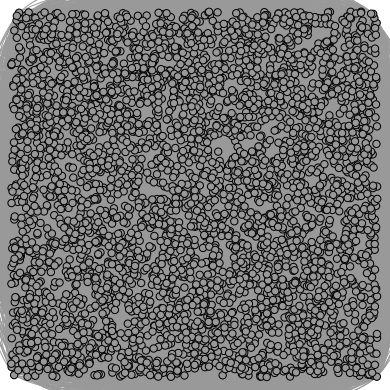
\includegraphics[height=7cm]{includes/snapshot_start}
		\end{figure}
    \end{frame}
    
    \begin{frame}{3.4 Visualisierung mit Gephi}{Grafik nach Anwendung von Layout-Algorithmen}
       \begin{figure}
    		\centering
    		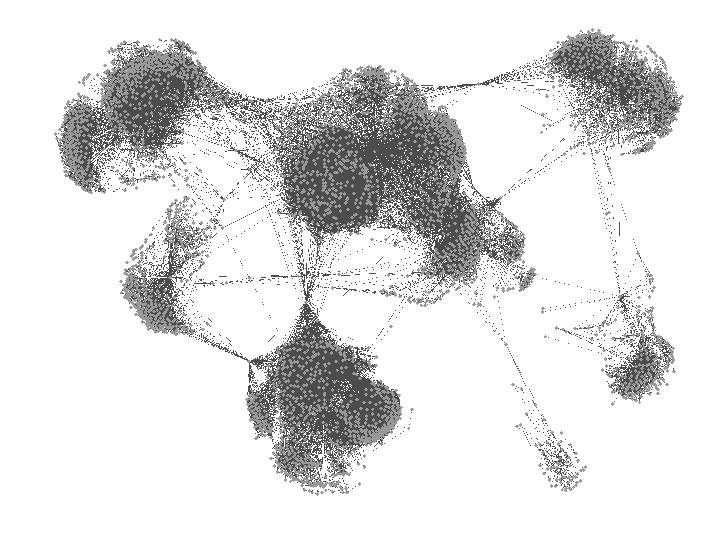
\includegraphics[height=7cm]{includes/snapshot_einfarbig}
		\end{figure}
    \end{frame}
    
    \begin{frame}{3.4 Visualisierung mit Gephi}{Grafik nach Anwendung von Layout-Algorithmen und Einfärben der Knoten}
       \begin{figure}
    		\centering
    		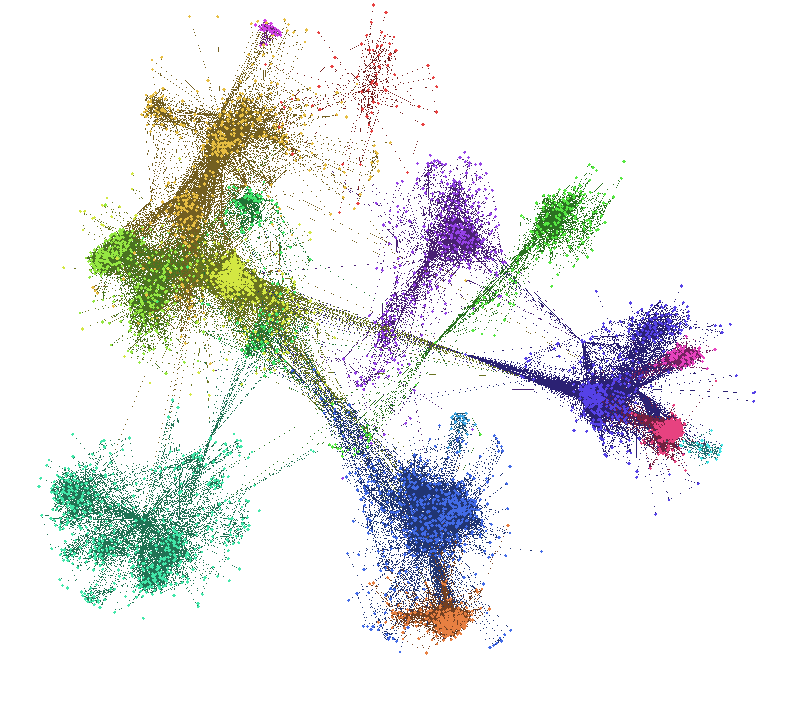
\includegraphics[height=7cm]{includes/snapshot_bunt}
		\end{figure}
    \end{frame}
    
    \begin{frame}{Informationsvisualisierung}{Übungspräsentation}
    	Vielen Dank für die Aufmerksamkeit.
    \end{frame}

\end{document}